%\documentclass[handout]{ximera}
\documentclass{ximera}

\usepackage{gensymb}
\usepackage{tabularx}
\usepackage{mdframed}
\usepackage{pdfpages}
%\usepackage{chngcntr}

\let\problem\relax
\let\endproblem\relax

\newcommand{\property}[2]{#1#2}




\newtheoremstyle{SlantTheorem}{\topsep}{\fill}%%% space between body and thm
 {\slshape}                      %%% Thm body font
 {}                              %%% Indent amount (empty = no indent)
 {\bfseries\sffamily}            %%% Thm head font
 {}                              %%% Punctuation after thm head
 {3ex}                           %%% Space after thm head
 {\thmname{#1}\thmnumber{ #2}\thmnote{ \bfseries(#3)}} %%% Thm head spec
\theoremstyle{SlantTheorem}
\newtheorem{problem}{Problem}[]

%\counterwithin*{problem}{section}



%%%%%%%%%%%%%%%%%%%%%%%%%%%%Jenny's code%%%%%%%%%%%%%%%%%%%%

%%% Solution environment
%\newenvironment{solution}{
%\ifhandout\setbox0\vbox\bgroup\else
%\begin{trivlist}\item[\hskip \labelsep\small\itshape\bfseries Solution\hspace{2ex}]
%\par\noindent\upshape\small
%\fi}
%{\ifhandout\egroup\else
%\end{trivlist}
%\fi}
%
%
%%% instructorIntro environment
%\ifhandout
%\newenvironment{instructorIntro}[1][false]%
%{%
%\def\givenatend{\boolean{#1}}\ifthenelse{\boolean{#1}}{\begin{trivlist}\item}{\setbox0\vbox\bgroup}{}
%}
%{%
%\ifthenelse{\givenatend}{\end{trivlist}}{\egroup}{}
%}
%\else
%\newenvironment{instructorIntro}[1][false]%
%{%
%  \ifthenelse{\boolean{#1}}{\begin{trivlist}\item[\hskip \labelsep\bfseries Instructor Notes:\hspace{2ex}]}
%{\begin{trivlist}\item[\hskip \labelsep\bfseries Instructor Notes:\hspace{2ex}]}
%{}
%}
%% %% line at the bottom} 
%{\end{trivlist}\par\addvspace{.5ex}\nobreak\noindent\hung} 
%\fi
%
%


\let\instructorNotes\relax
\let\endinstructorNotes\relax
%%% instructorNotes environment
\ifhandout
\newenvironment{instructorNotes}[1][false]%
{%
\def\givenatend{\boolean{#1}}\ifthenelse{\boolean{#1}}{\begin{trivlist}\item}{\setbox0\vbox\bgroup}{}
}
{%
\ifthenelse{\givenatend}{\end{trivlist}}{\egroup}{}
}
\else
\newenvironment{instructorNotes}[1][false]%
{%
  \ifthenelse{\boolean{#1}}{\begin{trivlist}\item[\hskip \labelsep\bfseries {\Large Instructor Notes: \\} \hspace{\textwidth} ]}
{\begin{trivlist}\item[\hskip \labelsep\bfseries {\Large Instructor Notes: \\} \hspace{\textwidth} ]}
{}
}
{\end{trivlist}}
\fi


%% Suggested Timing
\newcommand{\timing}[1]{{\bf Suggested Timing: \hspace{2ex}} #1}




\hypersetup{
    colorlinks=true,       % false: boxed links; true: colored links
    linkcolor=blue,          % color of internal links (change box color with linkbordercolor)
    citecolor=green,        % color of links to bibliography
    filecolor=magenta,      % color of file links
    urlcolor=cyan           % color of external links
}

\title{Trapezoid Area}
\author{Bart Snapp and Brad Findell}

\outcome{Learning outcome goes here.}

\begin{document}
\begin{abstract}
Abstract goes here.  
\end{abstract}
\maketitle


\begin{teachingnote}
Precede this with triangle area problems 1.3.7 and 8.  The point is connecting the geometric thinking with the algebraic thinking.  For example, how, algebraically and geometrically, does the first one look like an average?  In the last problem, students might not see the similar triangles.
\end{teachingnote}

\begin{problem}
In this activity, we explore several ways of justifying the formula for the area of a trapezoid, as labeled below. 
\begin{image}
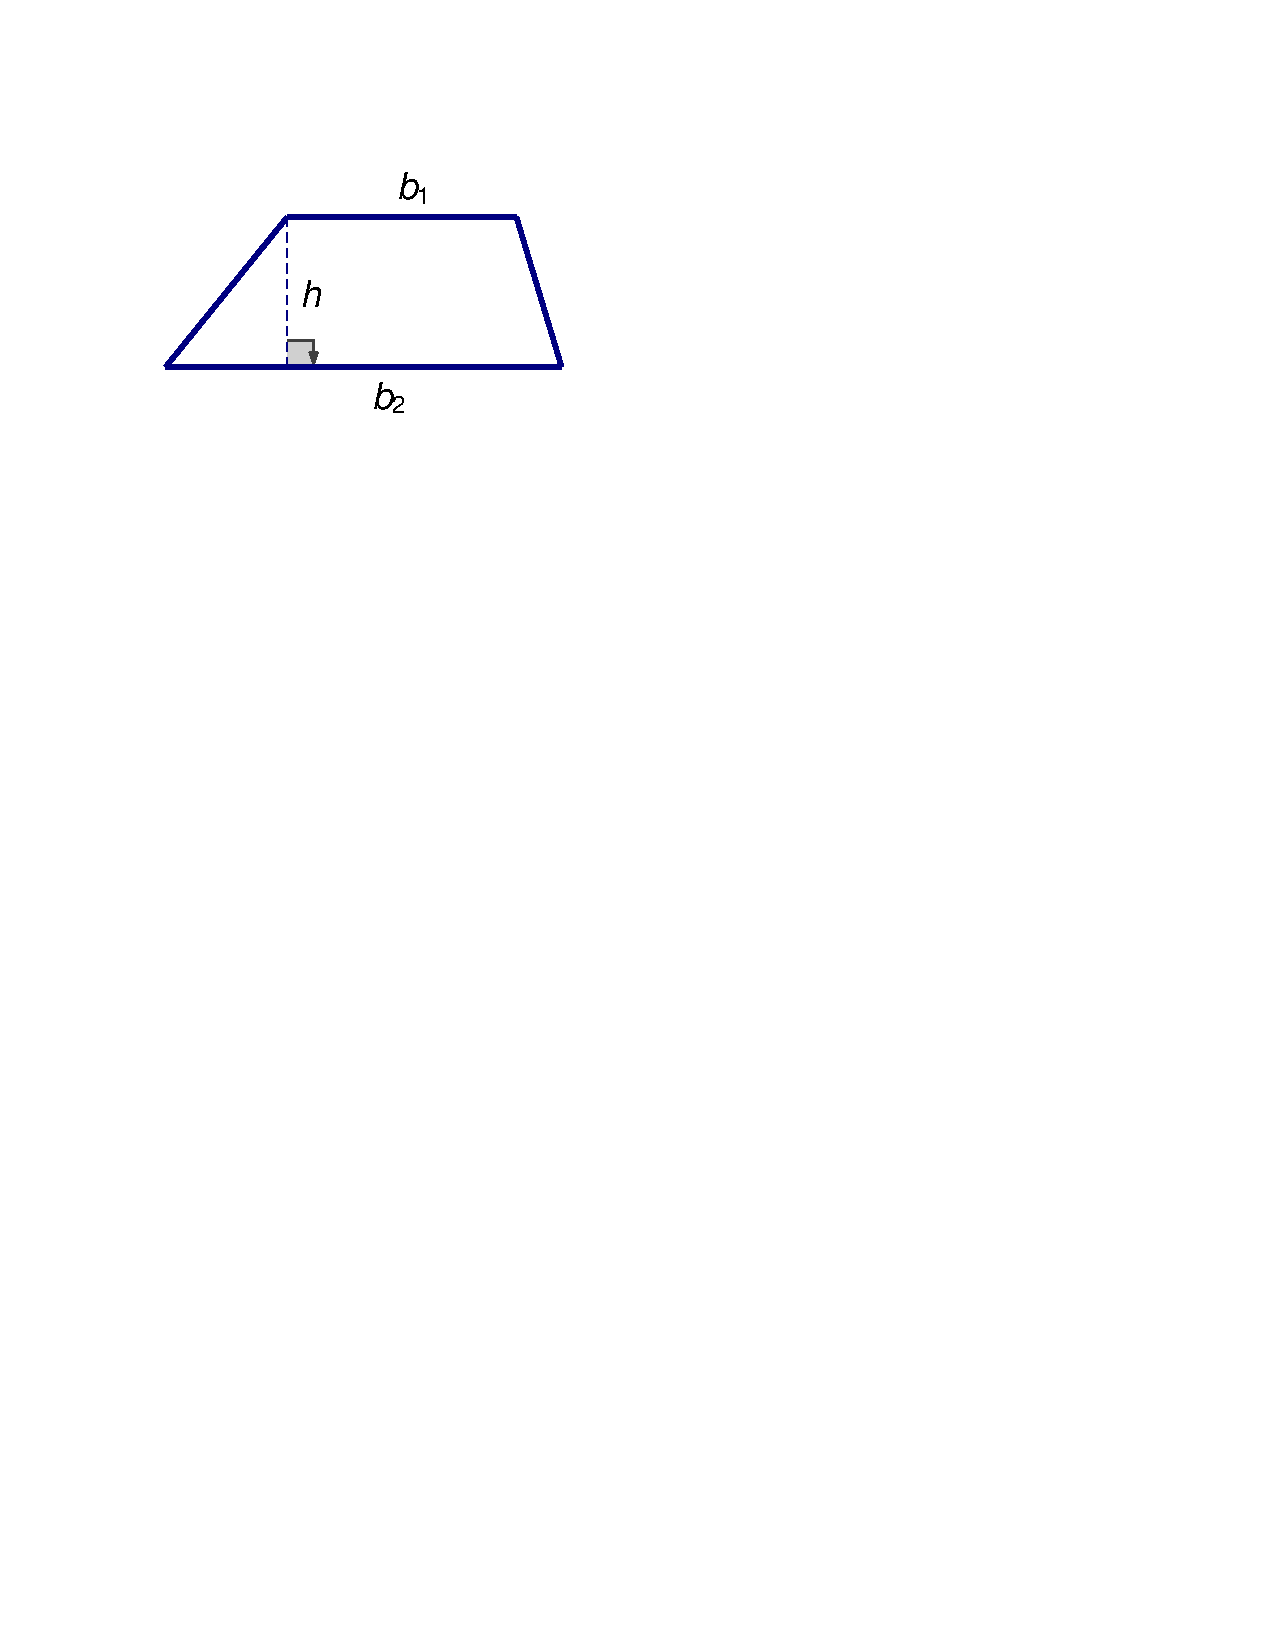
\includegraphics[scale=0.6]{trapezoid1.pdf}
\end{image}
Complete the table on the following page so that, in each row, the explanation, the geometric figure, and the algebraic formula together describe a way of computing the area.  For comparison purposes, each illustration should include a trapezoid congruent to the trapezoid above.   

All of the area formulas will, of course, be equivalent to one another as expressions.  But each way of expressing the area will make the most sense with figure and the explanation from the same row.  

\begin{teachingnote}
The next page is for students and then a completed answer page follows.
\end{teachingnote}

\fixnote{For the student edition, comment out the answer page.  For the teacher edition, uncomment.}


\newpage

\newlength{\formulawidth}
\settowidth{\formulawidth}{$\frac{1}{2}b_2(x+h)-\frac{1}{2}b_1x$, with $\frac{x}{b_1}=\frac{x+h}{b_2}$}  
\resizebox{\textwidth}{!}{
{\renewcommand{\arraystretch}{1.5}
\begin{tabular}{|>{\centering\arraybackslash}m{2.5cm}|>{\centering\arraybackslash}m{9.5cm}|c|}\hline
Explanation & Figure & Area Formula \\\hline

Rectangle with width that is the average of the bases. & 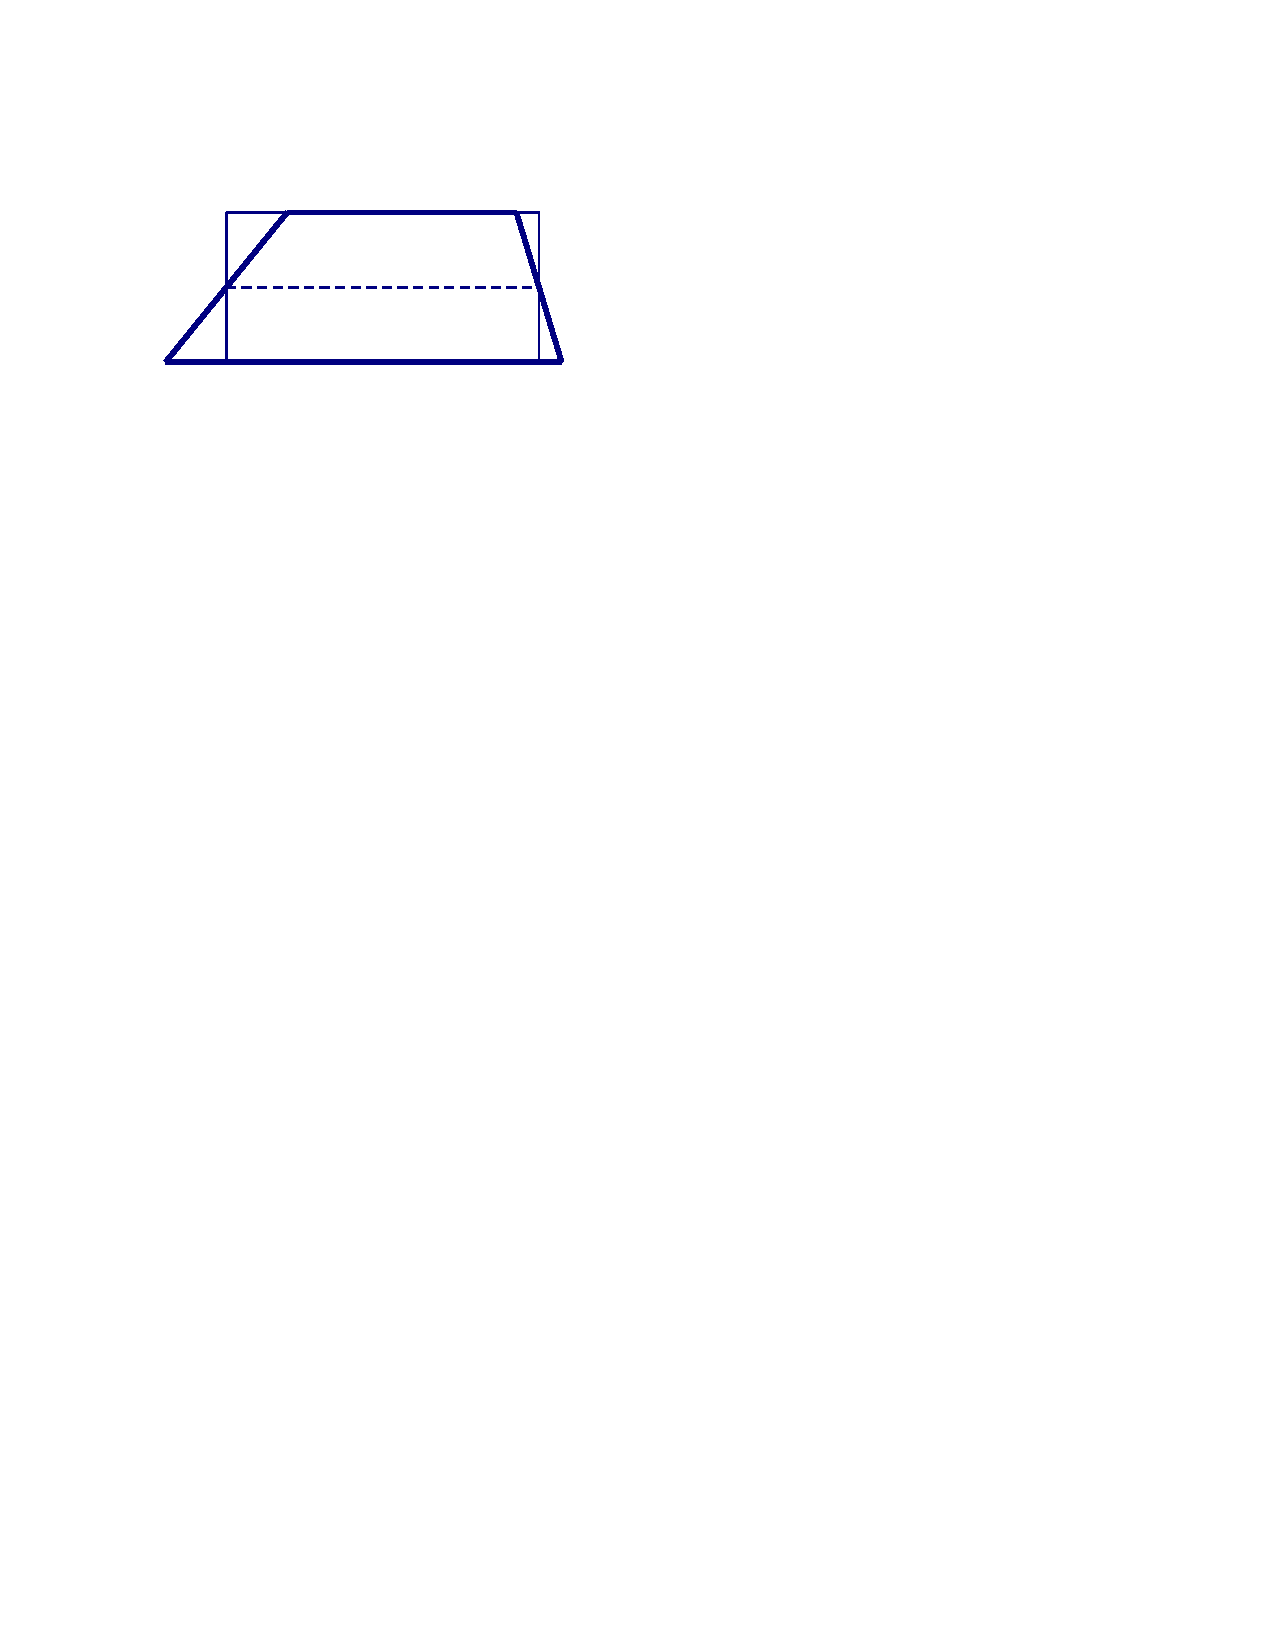
\includegraphics[scale=0.7]{trapezoid2.pdf} & $\left(\frac{b_1+b_2}{2}\right)h$ \\ \hline
                              & 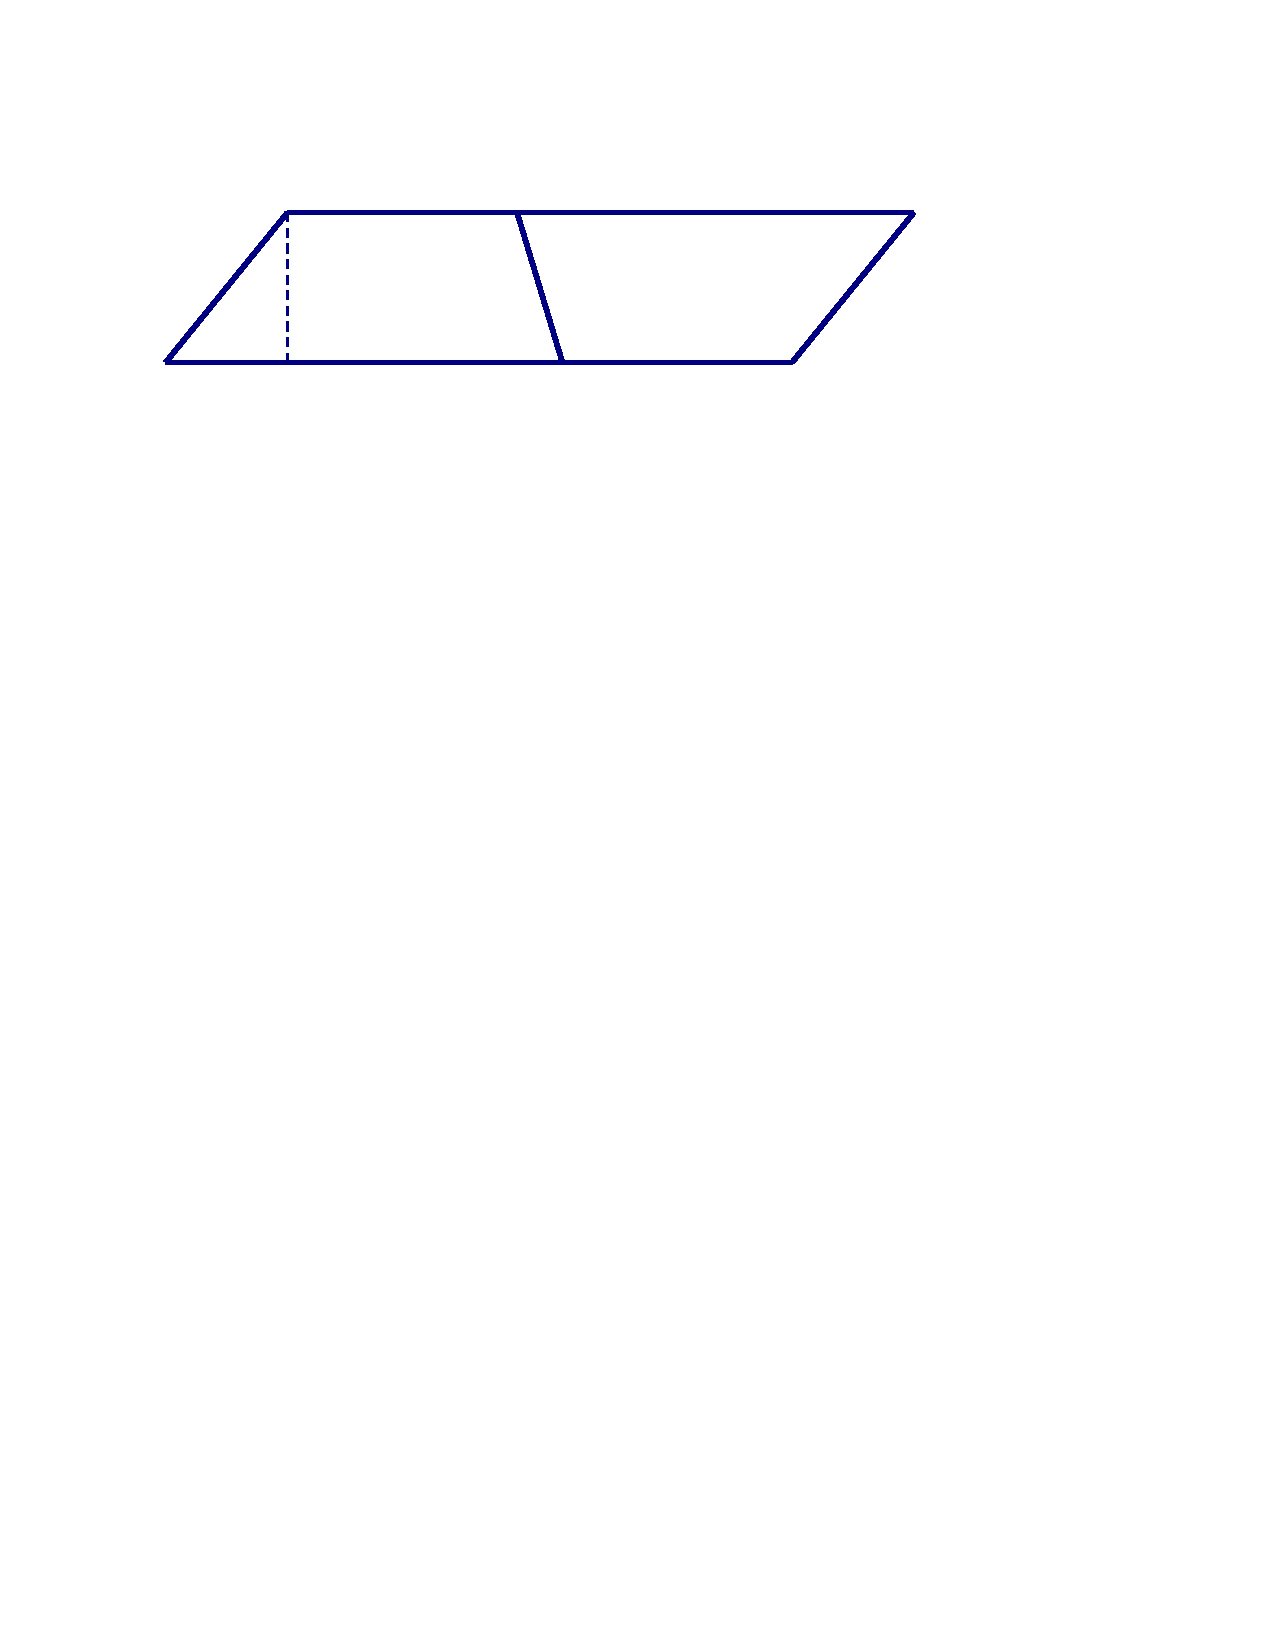
\includegraphics[scale=0.7]{trapezoid3.pdf} &                      \\ \hline
Two triangles with the same height and different bases. &                 & \\ \hline
 & & \\ 
\bigskip                              &  & $(b_1+b_2)\frac{h}{2}$ \\ 
 & & \\ \hline
          & 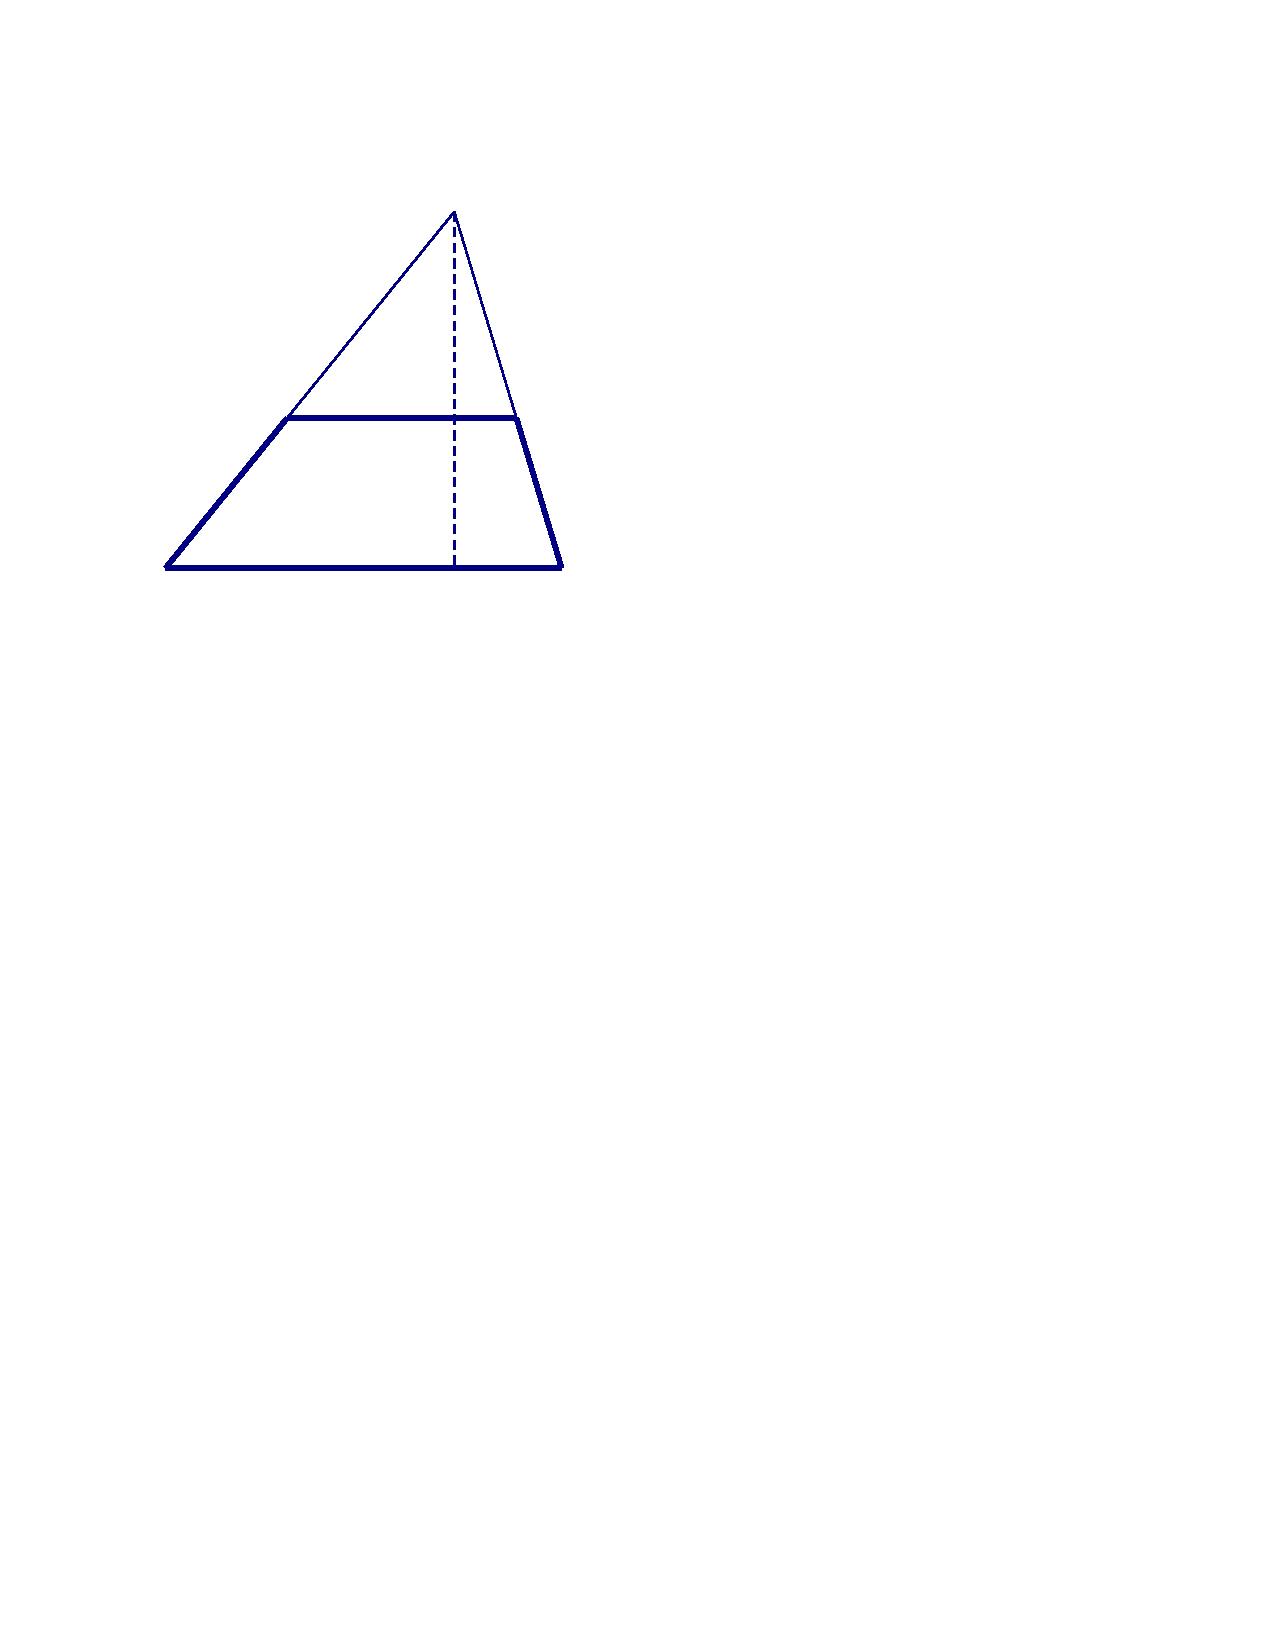
\includegraphics[scale=0.7]{trapezoid6.pdf}&  \hspace{\formulawidth} \\ \hline
\end{tabular}}
}

\end{problem}

%
%   Answers  (Comment out the following lines for student edition)
%
\newpage
\resizebox{\textwidth}{!}{
{\renewcommand{\arraystretch}{1.5}
\begin{tabular}{|>{\centering\arraybackslash}m{2.5cm}|>{\centering\arraybackslash}m{9.5cm}|c|}\hline
Explanation & Figure & Area Formula \\\hline

Rectangle with width that is the average of the bases. & 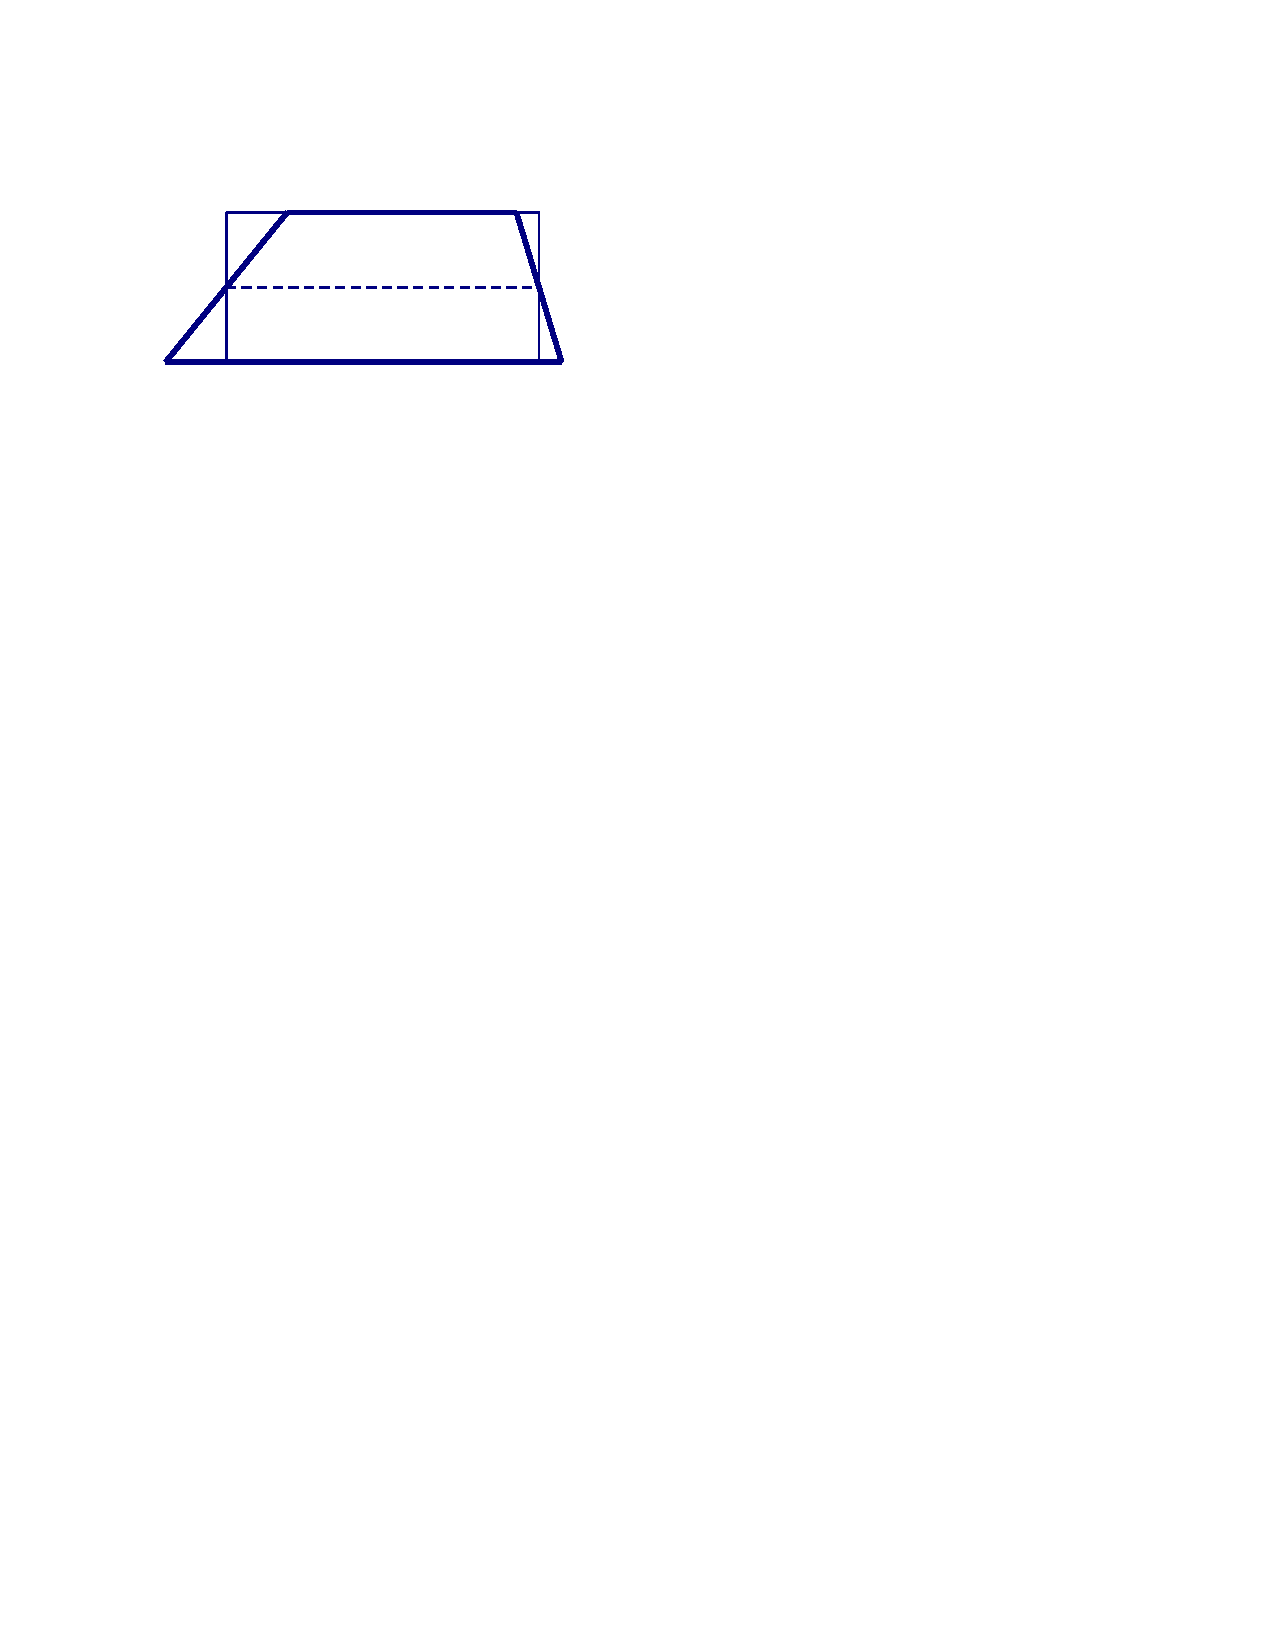
\includegraphics[scale=0.7]{trapezoid2.pdf} & $\left(\frac{b_1+b_2}{2}\right)h$ \\ \hline
Half of a large parallelogram. & 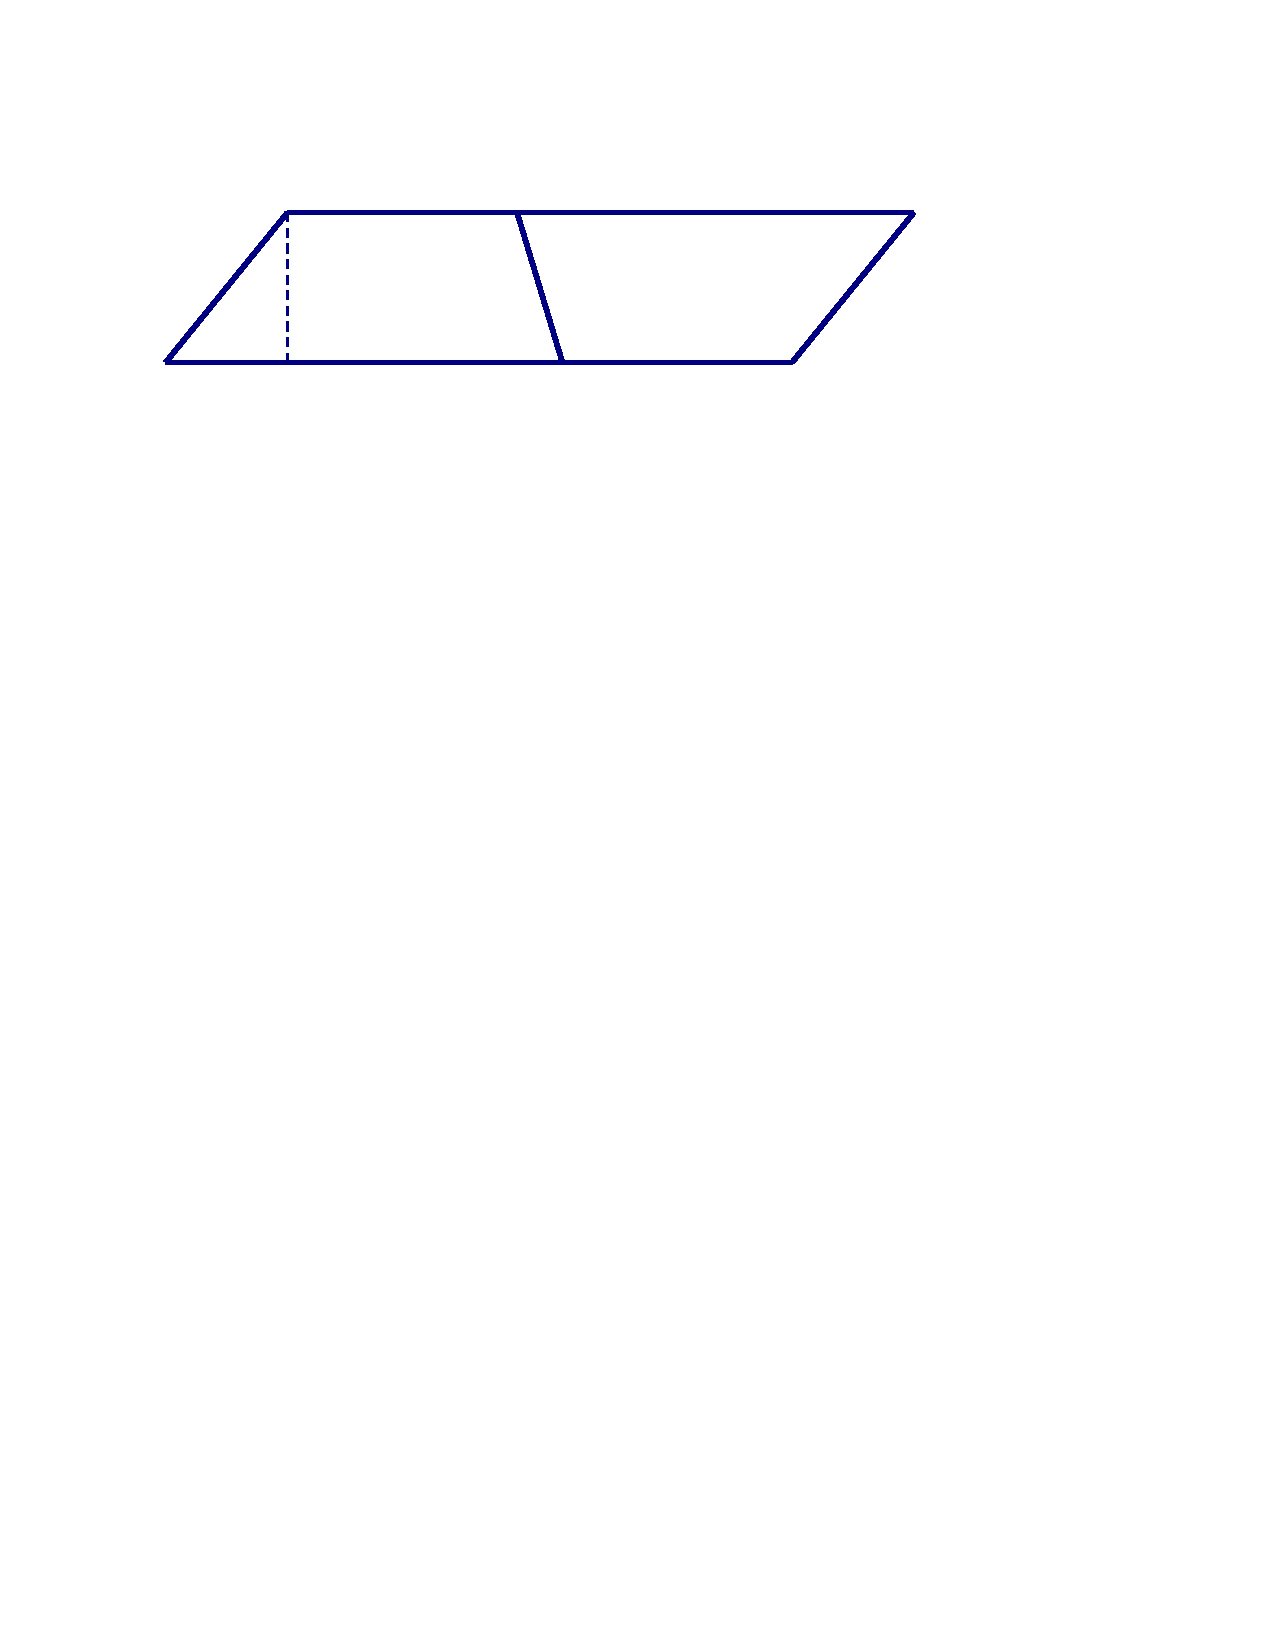
\includegraphics[scale=0.7]{trapezoid3.pdf} & $\frac{1}{2}(b_1+b_2)h$ \\ \hline
Two triangles with the same height and different bases. & 
\includegraphics[scale=0.7]{trapezoid4.pdf} & $\frac{1}{2}b_1h + \frac{1}{2}b_2h$ \\ \hline
A parallelogram with half the height. & 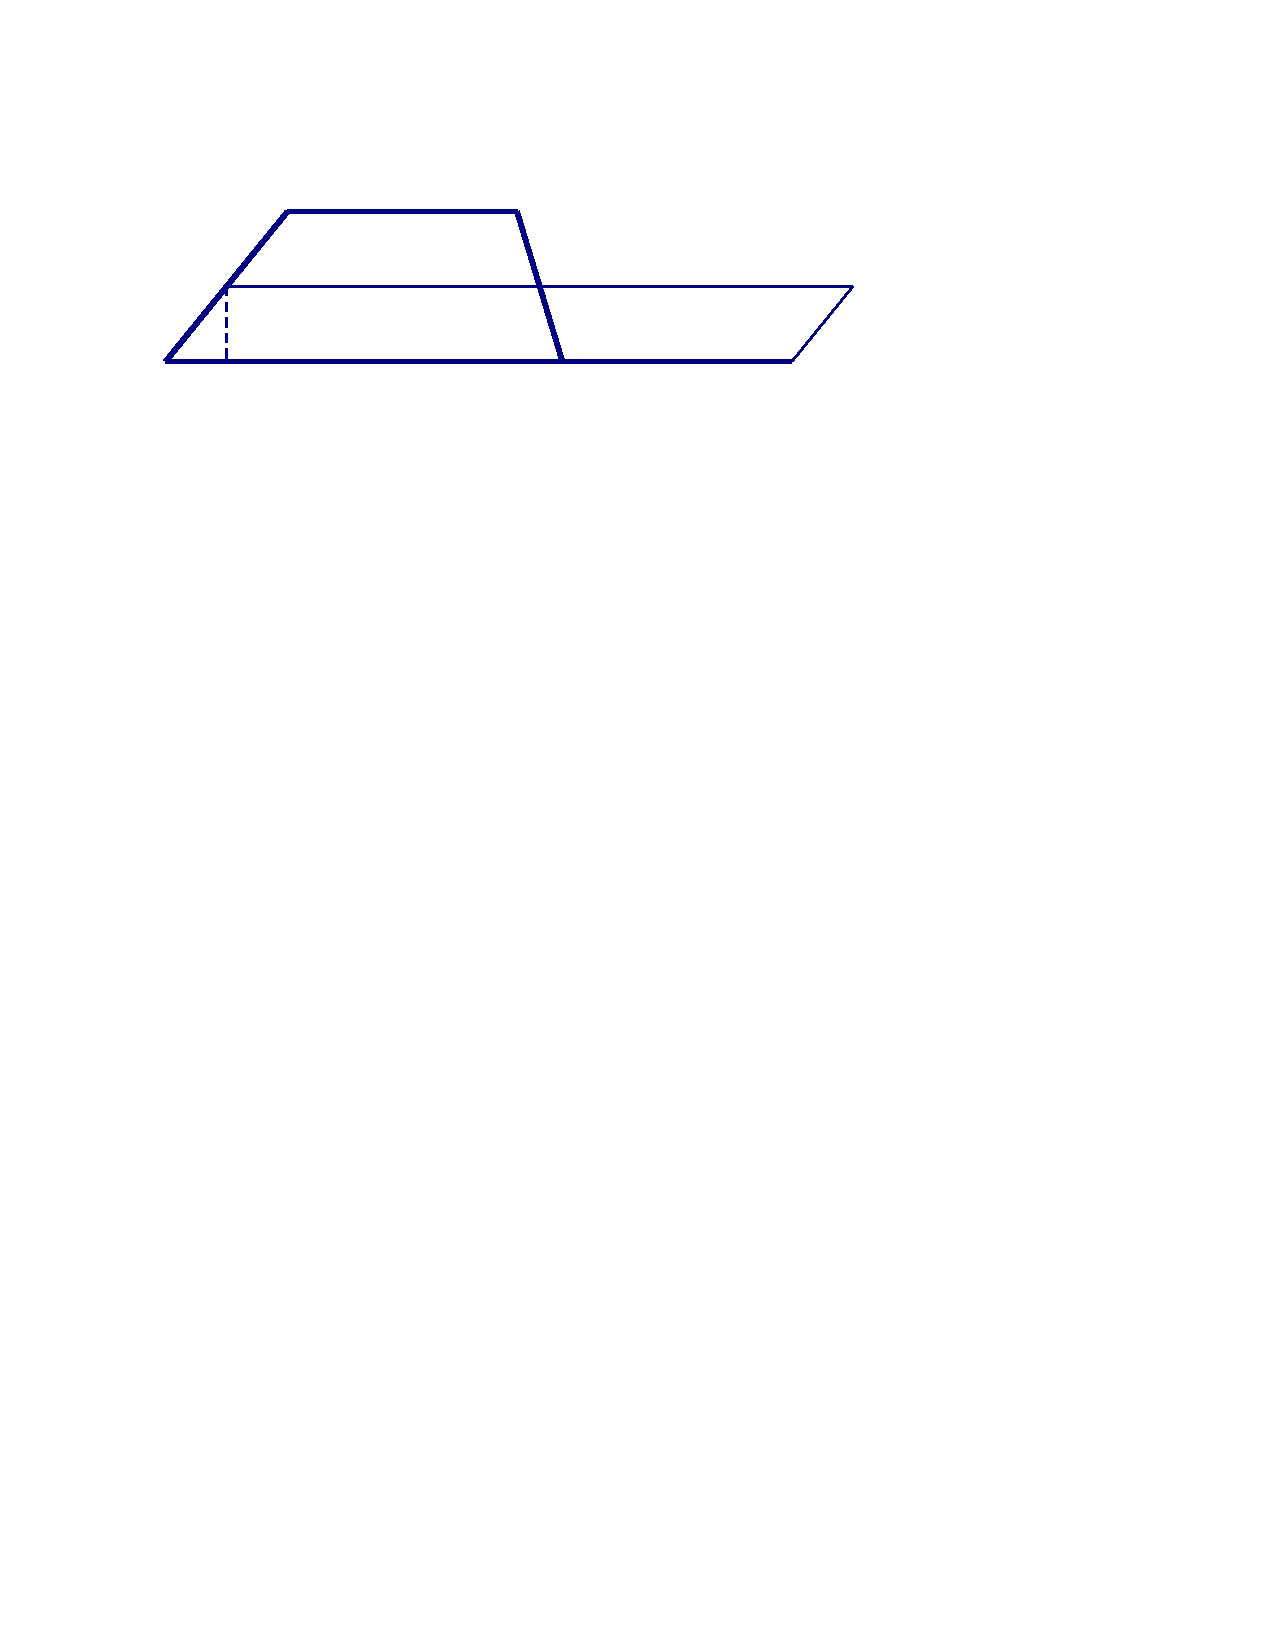
\includegraphics[scale=0.7]{trapezoid5.pdf} & $(b_1+b_2)\frac{h}{2}$ \\ \hline
Difference between two triangles, with $x$ as height of small triangle. 
          & 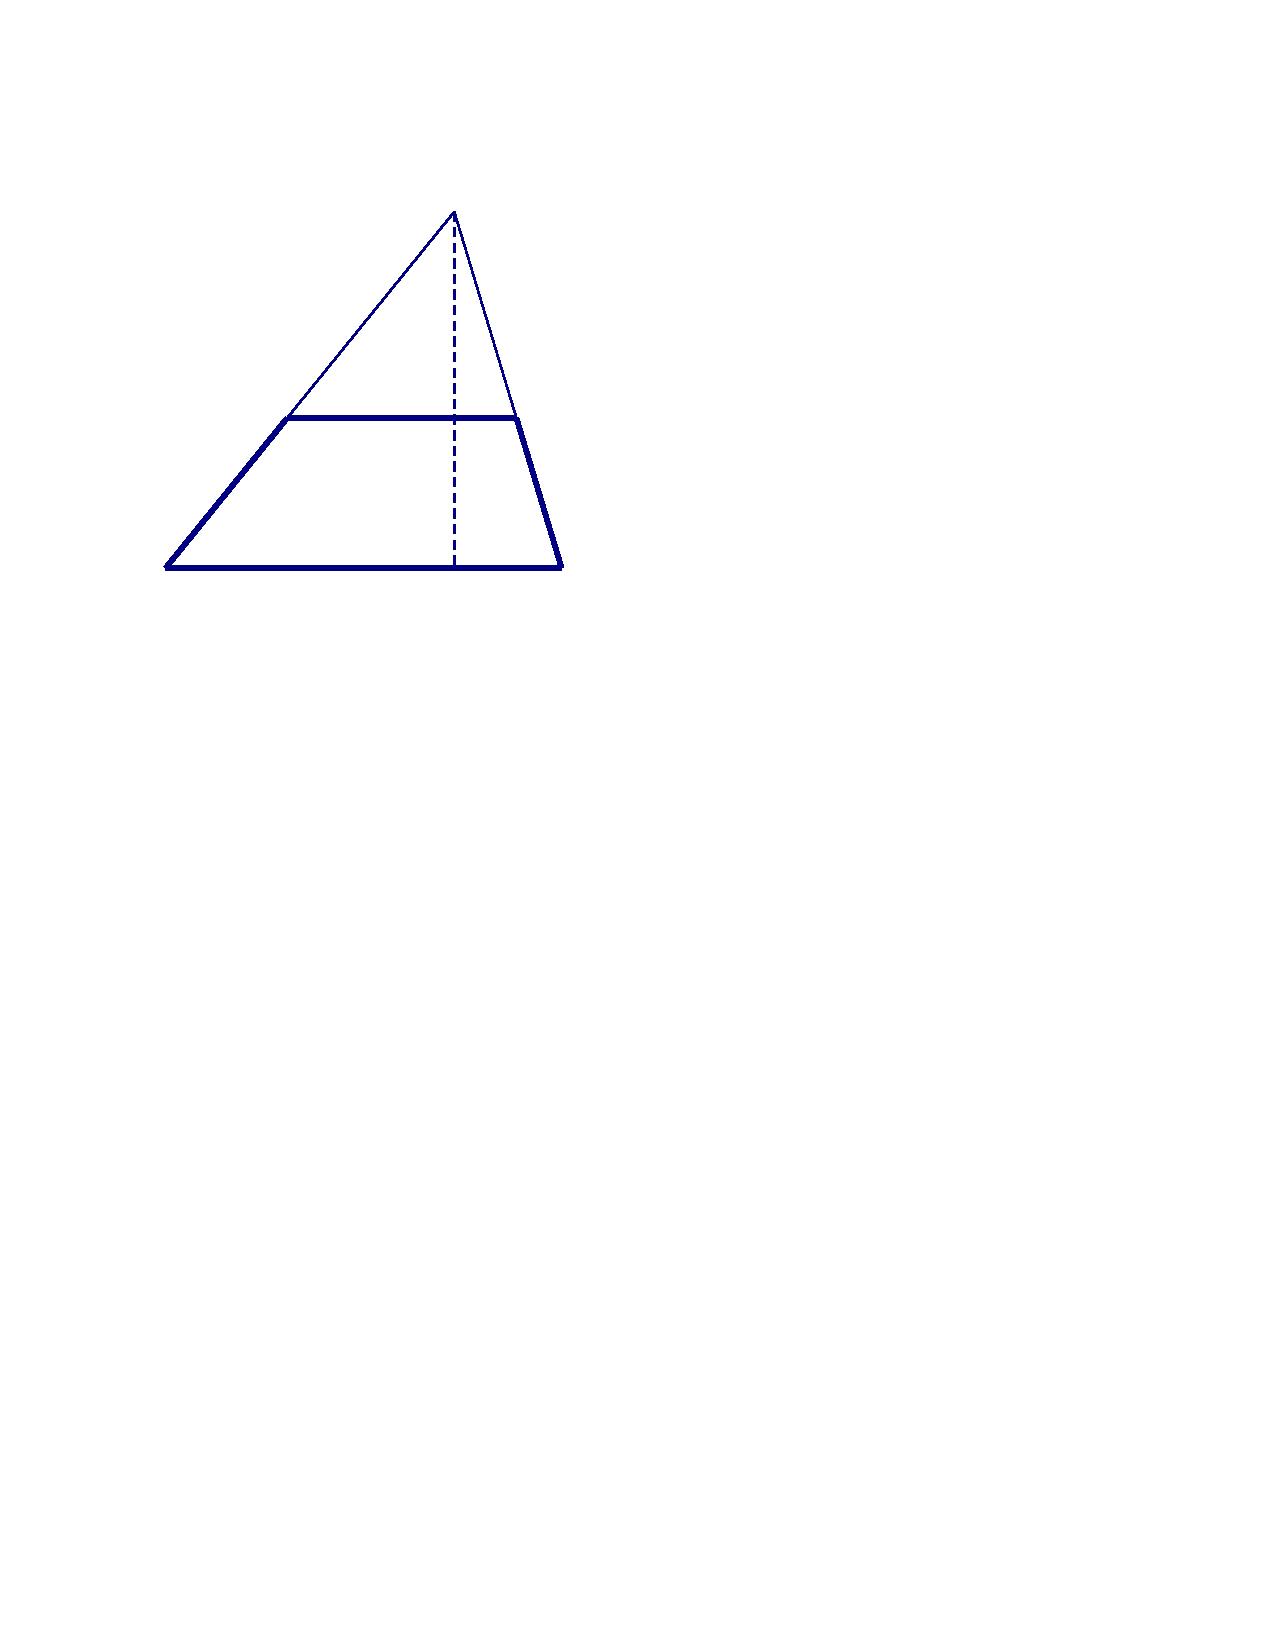
\includegraphics[scale=0.7]{trapezoid6.pdf} &  $\frac{1}{2}b_2(x+h)-\frac{1}{2}b_1x$, with $\frac{x}{b_1}=\frac{x+h}{b_2}$ \\ \hline
\end{tabular}}
}
\end{document}
